%----------------------------------------------------------------------------------------
% Analisi del contesto
%----------------------------------------------------------------------------------------

\documentclass[10pt]{softeng} % Document font size and equations flushed left

%----------------------------------------------------------------------------------------
%	ARTICLE INFORMATION
%----------------------------------------------------------------------------------------

\Phase{Inception - I iterazione} % Additional notes (e.g. copyright, DOI, review/research article)

\DocumentTitle{Analisi del contesto e studio di fattibilit\`a} % Article title

%----------------------------------------------------------------------------------------

\begin{document}

\startofdocument{}

\section{Collocazione del progetto}

% intenzione progetto, collocazione

\section{Analisi del contesto}

Chiamiamo ``utente registrato (al sistema di Home Banking della banca X)'' una persona fisica titolare di un account di Home Banking all'interno del sistema di una particolare banca, e che quindi abbia fornito informazioni anagrafiche e di contatto, e eventualmente informazioni non obbligatorie sulla sua condizione economica e famigliare.

Chiamiamo ``utente titolare di un conto corrente'' un utente registrato presso la banca X che abbia ultimato la procedura di autenticazione della suddetta banca.

Il bonifico \`e un trasferimento di denaro da un conto corrente a un altro.
Un utente titolare di un conto corrente pu\`o effettuare bonifici dal suo conto corrente.
Distinguiamo due tipi di bonifici:
\begin{itemize}
	\item Bonifico Italia se il conto corrente destinatario \`e aperto presso una banca italiana.
	Per effettuare un Bonifico Italia \`e necessario conoscere nome, cognome, indirizzo e codice IBAN del destinatario.
	\item Bonifico SEPA se il conto corrente destinatario \`e aperto presso una banca europea. Per effettuare un Bonifico SEPA \`e necessario conoscere anche il codice BIC/SWIFT della banca del destinatario \cite{bonifico_unicredit}.
\end{itemize}
Poich\'e la maggioranza dei pagamenti che una persona deve effettuare (tasse, bollette, ricariche, etc.) avvengono tramite bonifico, utenti di un sistema di Home Banking ritengono utile la possibilit\`a di effettuare pagamenti di un certo tipo tramite ``maschere specializzate'', che facilitino la compilazione dei dati e aiutino l'utente a evitare errori.

\subsection{Certificati di deposito}

% TODO scrivere qualcosa o togliere

\subsection{Portafoglio fondi}

La gestione di un portafoglio fondi \`e un argomento complesso.

Le norme che regolano l'acquisto di azioni e le procedure necessarie per acquisire dati aggiornati sull'andamento dei titoli esulano dalla portata di questo progetto, ricadendo nell'area di competenza del \emph{trading online}, e non dell'Home Banking.

% TODO espandere: fare tutto \`e infattibile, riduciamo roba da fare
% al max gli utenti vedono i fondi e possono venderli

\subsection{Legislazione taliana}

La Banca d'Italia si occupa di esercitare ``l'attivit\`a di vigilanza sulle banche'', e ``ha funzioni di controllo in materia di antiriciclaggio'' \cite[Funzioni]{banca_italia}.

% TODO espandere: cosa serve

\section{Fattibilit\`a}

Obiettivo del progetto \`e la realizzazione di un software di Home Banking, i cui utenti sono unicamente persone fisiche.
Un software di Home Banking deve (idealmente) permettere all'utente di effettuare via internet tutte le operazioni che pu\`o normalmente effettuare allo sportello della sua banca.

Il sistema home banking \`e accessibile tramite un semplice browser web, e non richiede software aggiuntivo.
D'altronde l'utilizzo di tecnologie come TLS e HTTPS permette di rendere sicura la connessione per poter trasmettere le informazioni sensibili in modo sicuro.

Per motivi di sicurezza, legislativi, burocratici e tecnologici non \`e possibile effettuare ogni operazione via internet.
Un sistema di Home Banking effettuer\`a quindi un sottoinsieme proprio di queste operazioni.

Il nostro software cerca di fornire all'utente un mezzo semplice ed intuitivo per poter effettuare le operazioni bancarie quotidiane senza doversi recare alla banca.

Le banche target del nostro prodotto sono banche di taglia piccola, che a seguito dell'entrata in vigore dello standard OBP si troveranno sprovviste di sistema informatico. Il nostro prodotto permette loro di effettuare la transizione senza subire ``downtime''.

Definiamo il nostro software ``Small Bank Friendly'' in quanto:
\begin{itemize}
    \item Il software non viene sviluppato ``from scratch'' individualmente per ogni cliente, ci\`o riduce notevolmente il costo unitario.
    \item Il proggetto parte con l'idea di separare ed isolare le componenti rendendo il sistema adatto al deployment su cloud, evitando l'acquisto di hardware aggiuntivo.
    \item Il supporto per la banca \`e fornito dalla nostra societ\`a.
    \item Il supporto per gli utenti \`e fornito dalla nostra societ\`a (o partner di essa)
\end {itemize}

Questa impostazione permete al prodotto di essere competitivo dal punto di vista del prezzo, i costi di servizio di supporto vengono distribuiti fra pi\`u clienti. Inoltre una banca pu\`o far crescere il proprio sistema home banking in maniera incrementale: acquistando prima il minimo indispensabile e aggiungendo moduli a piacere in seguito.

D'altro canto l'uso di componenti aggiuntive permette al nostro sistema di soddisfare le esigenze di ogni banca, piccola o grande che si\`a.

\`E imperativo dispiegare il sistema il prima possibile, per questo motivo si \`e deciso di individuare e realizzare in primis le funzionalit\`a \emph{core}, postponendo lo sviluppo delle funzionalit\`a meno vitali, che possono essere integrate tramite componeti aggiuntive in seguito.

Dato che l'insieme delle funzionalit\`a core \`e relativamente piccolo e restringibile a piacere, si d\`a per scontato la fattibilit\`a.

Perch\'e lo sforzo di sviluppo sia ripagato \`e per\`o necessario che l'insieme di operazioni offerte dal sistema sia sufficientemente ampio da:
\begin{enumerate}
	\item soddisfare le esigenze della maggioranza degli utenti;
	\item essere generale al punto da fornire tutti i principali servizi di cui la banca che utilizza il software ha bisogno.
\end{enumerate}
L'effettiva fattibilit\`a viene quindi da una combinazione delle due considerazioni.

Inoltre una banca potrebbe esigere una funzionalit\`a non inizialmente prevista, per mitigare questa eventualit\`a il servizio post vendita dedica un team di specialisti di ``plugin development''.

Attualmente la quasi totalit\`a banche dispongono di un sistema di Home Banking.
L'introduzione dello standard OBP rende per\`o tutti questi sistemi obsoleti.
Il nostro progetto soddisfa un mercato che avr\`a bisogno in tempi brevi di un nuovo sistema di Home Banking.
Inoltre un software di Home Banking modulare e facilmente personalizzabile pu\`o essere adattato alle esigenze di pi\`u banche con \emph{refactoring} minimo, e quindi a costi ridotti.

\subsection{Requisiti minimi}

Abbiamo individuato i seguenti requisiti minimi, che riteniamo essere sufficienti a soddisfare le necessit\`a di buona parte delle banche.

% TODO espandere e copiare da documento requisiti

\subsection{Fattibilit\`a economica}

% TODO inserire info su why il progetto pu\`o avere un guadagno

\section{Conclusioni}

Riteniamo sia fattibile, con le limitazioni indicate, realizzare un sistema di Home Banking all'avanguardia, manutenibile, espandibile e generale.

%----------------------------------------------------------------------------------------
%	CHANGELOG
%----------------------------------------------------------------------------------------

\section{Registro modifiche}

\subsection{Inception}

\subsubsection{I iterazione}

Prima stesura documento.

%----------------------------------------------------------------------------------------
%	REFERENCE LIST
%----------------------------------------------------------------------------------------

\printcustombibsmall{}

%----------------------------------------------------------------------------------------
%	FIGURES
%----------------------------------------------------------------------------------------

\begin{figure*}[hbt]
	\centering
	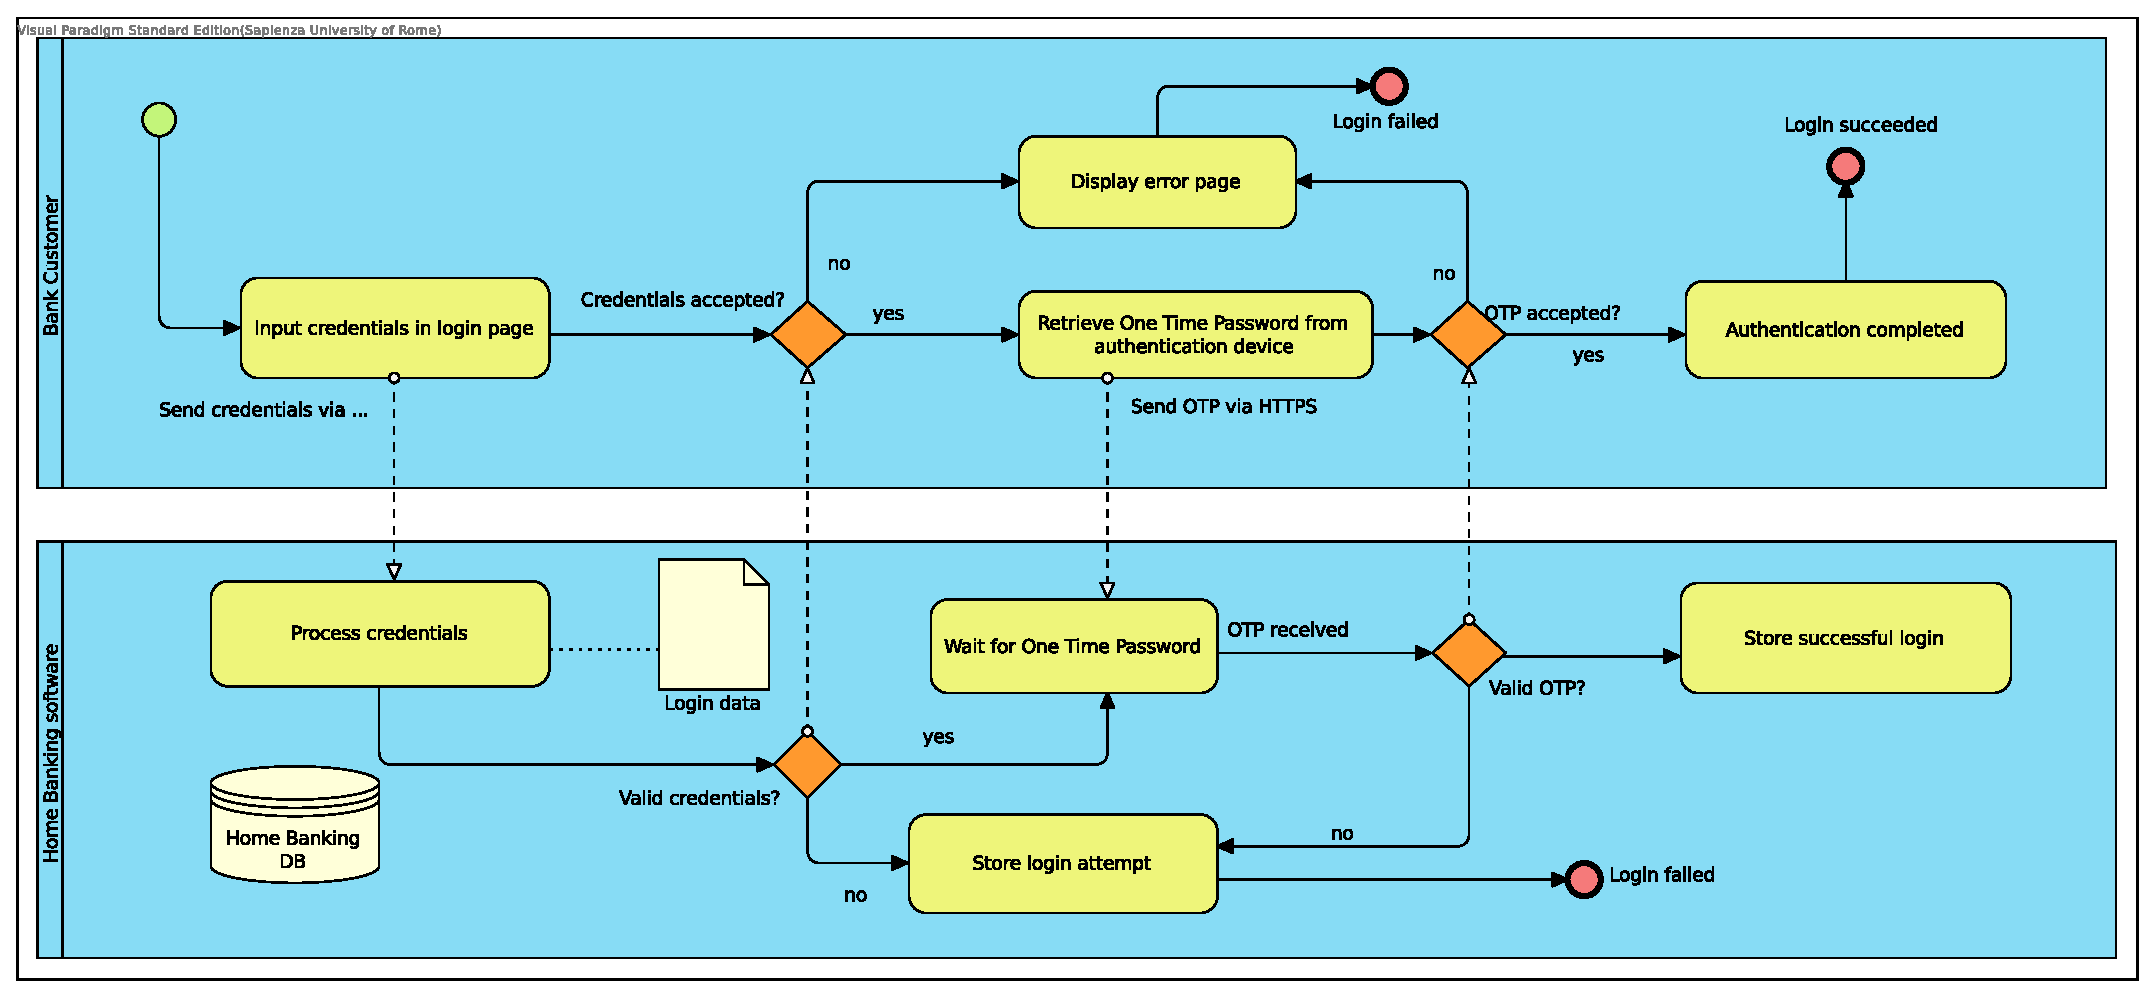
\includegraphics[width=\textheight, angle=90]{Images/Authentication.eps}
	\caption{Business case: procedura di autenticazione.}
	\label{fig:business_case_authentication}
\end{figure*}

\begin{figure*}[hbt]
	\centering
	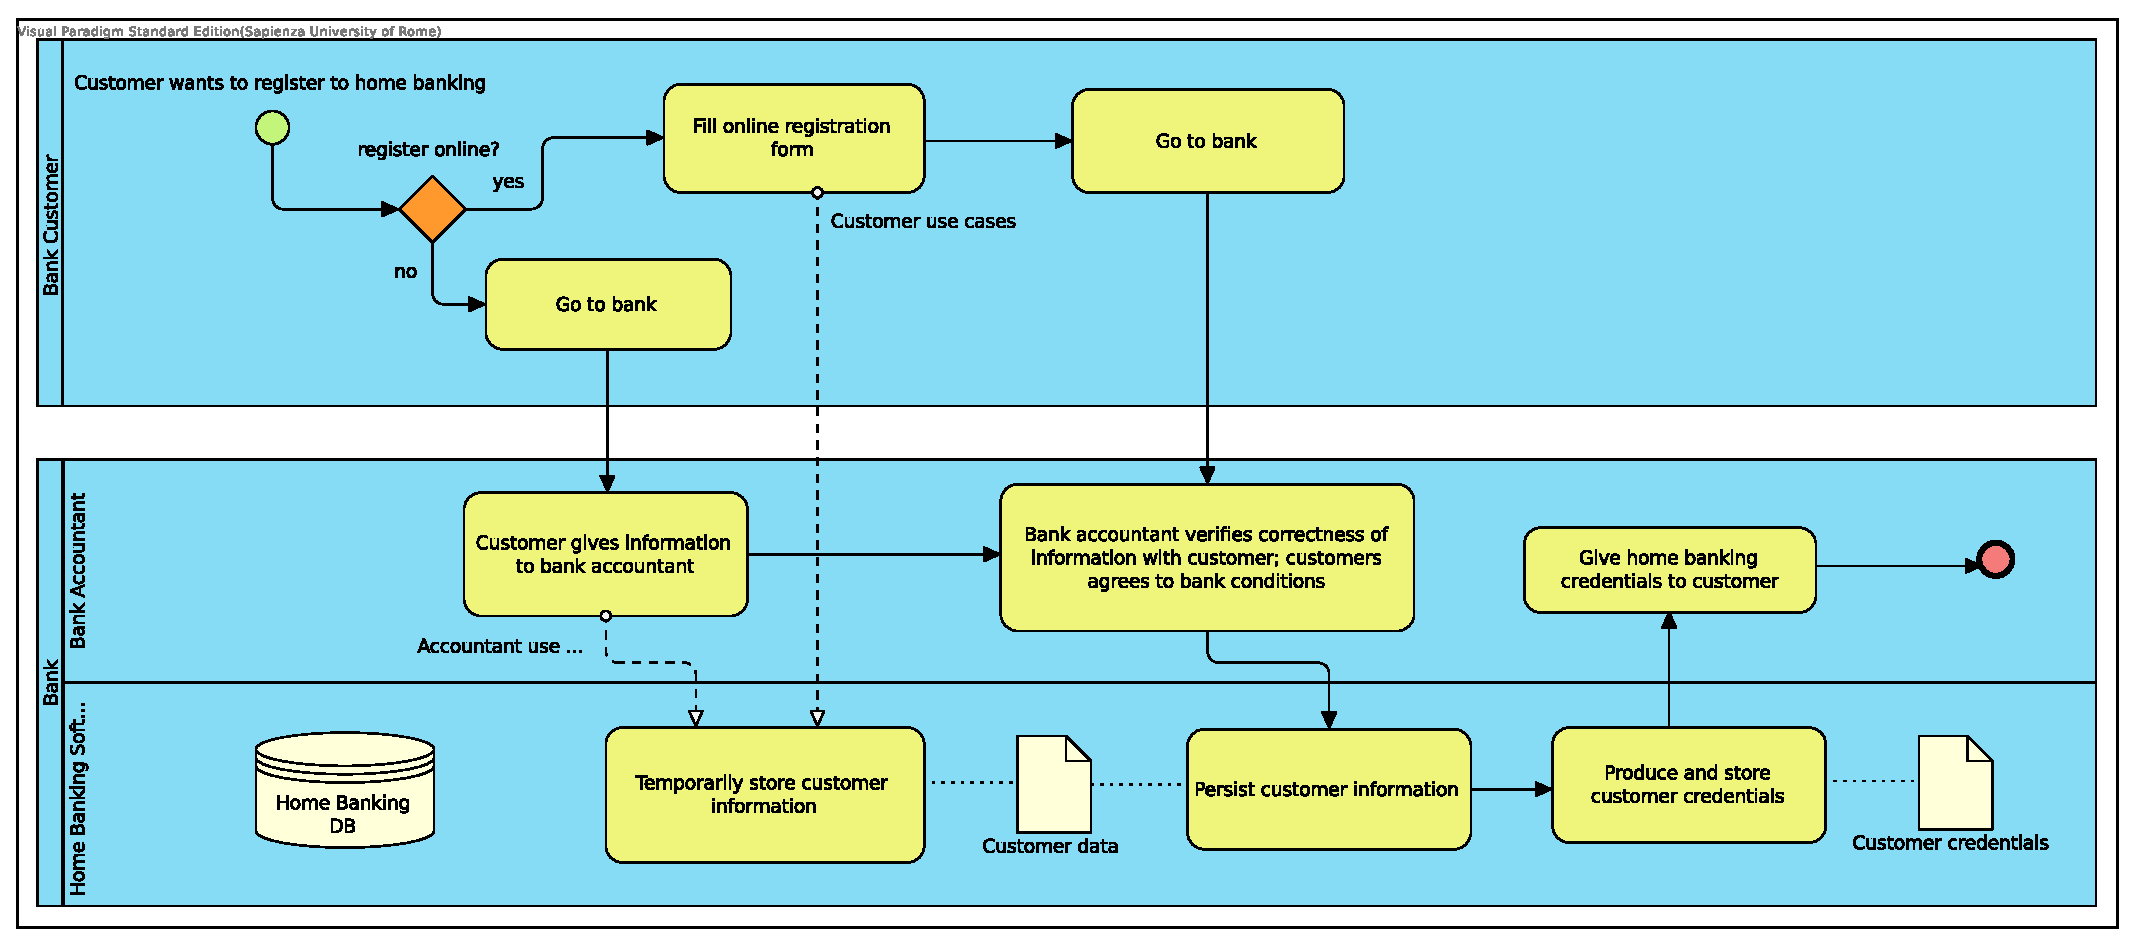
\includegraphics[width=\textheight, angle=90]{Images/Home_Banking_registration.eps}
	\caption{Business case: procedura di registrazione.}
	\label{fig:business_case_registration}
\end{figure*}

\begin{figure*}[hbt]
	\centering
	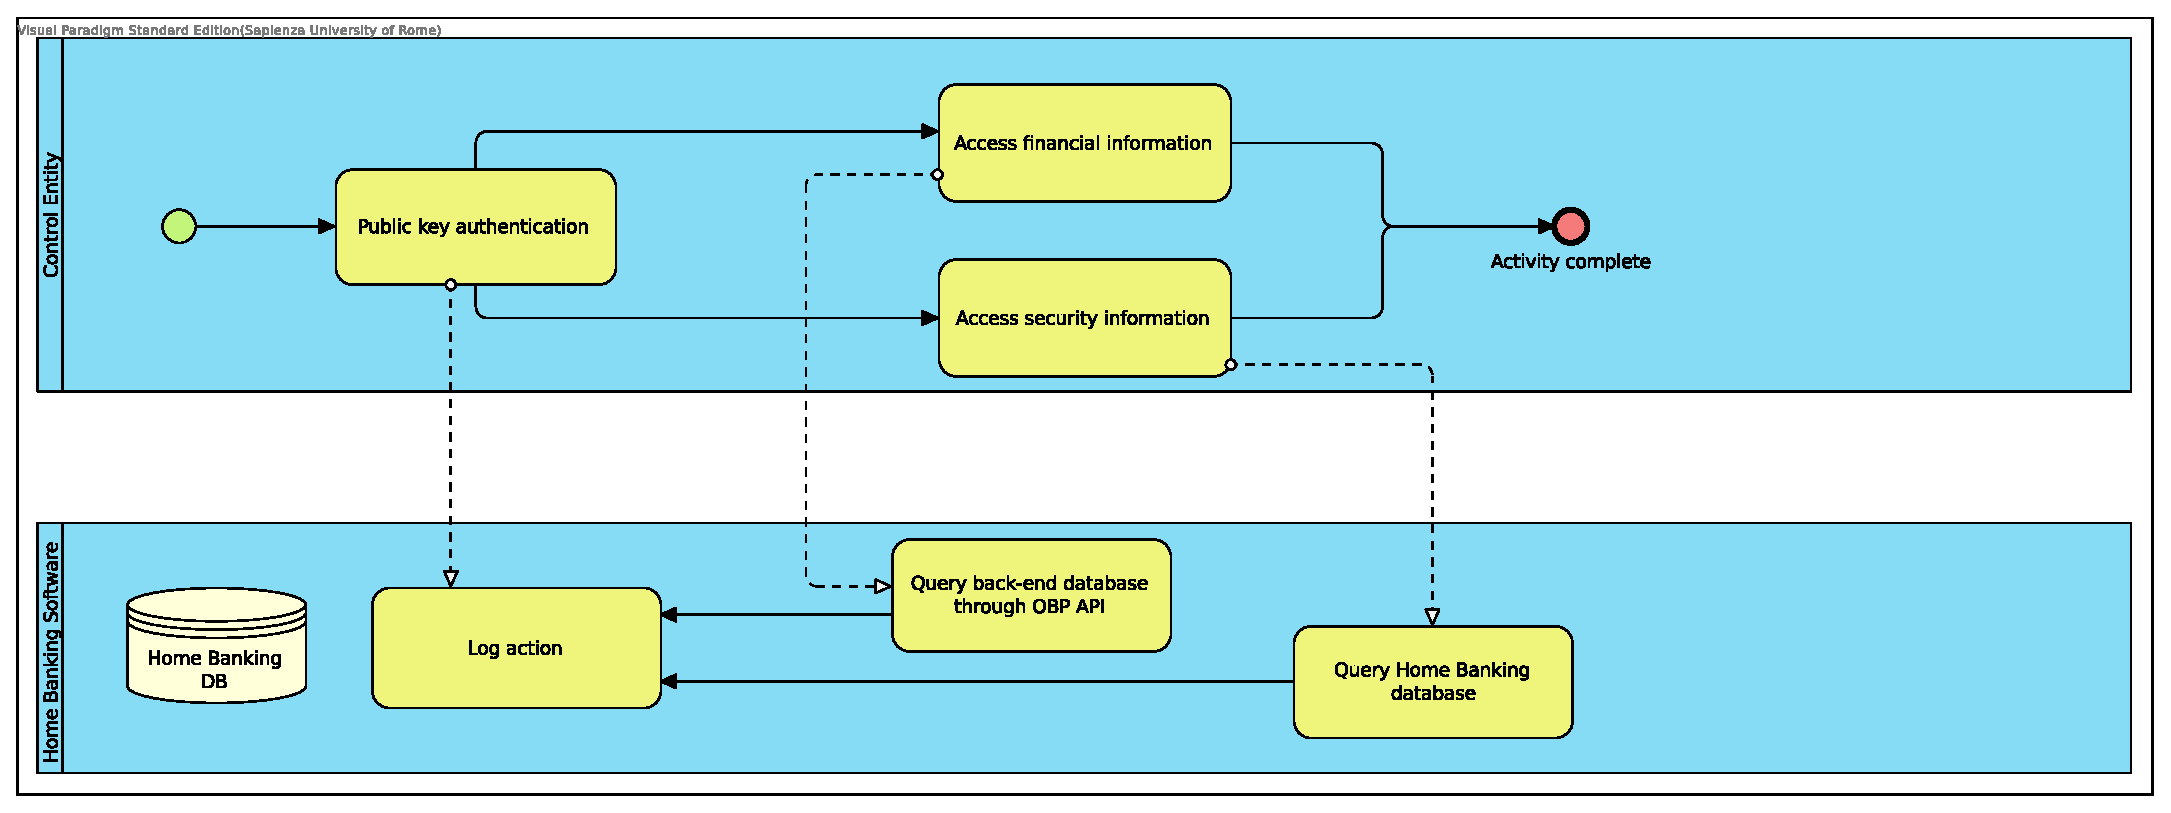
\includegraphics[width=\textheight, angle=90]{Images/Home_Banking_control_activity.eps}
	\caption{Business case: attivit\`a di controllo effettuata da enti responsabili.}
	\label{fig:business_case_control_activity}
\end{figure*}

\begin{figure*}[hbt]
	\centering
	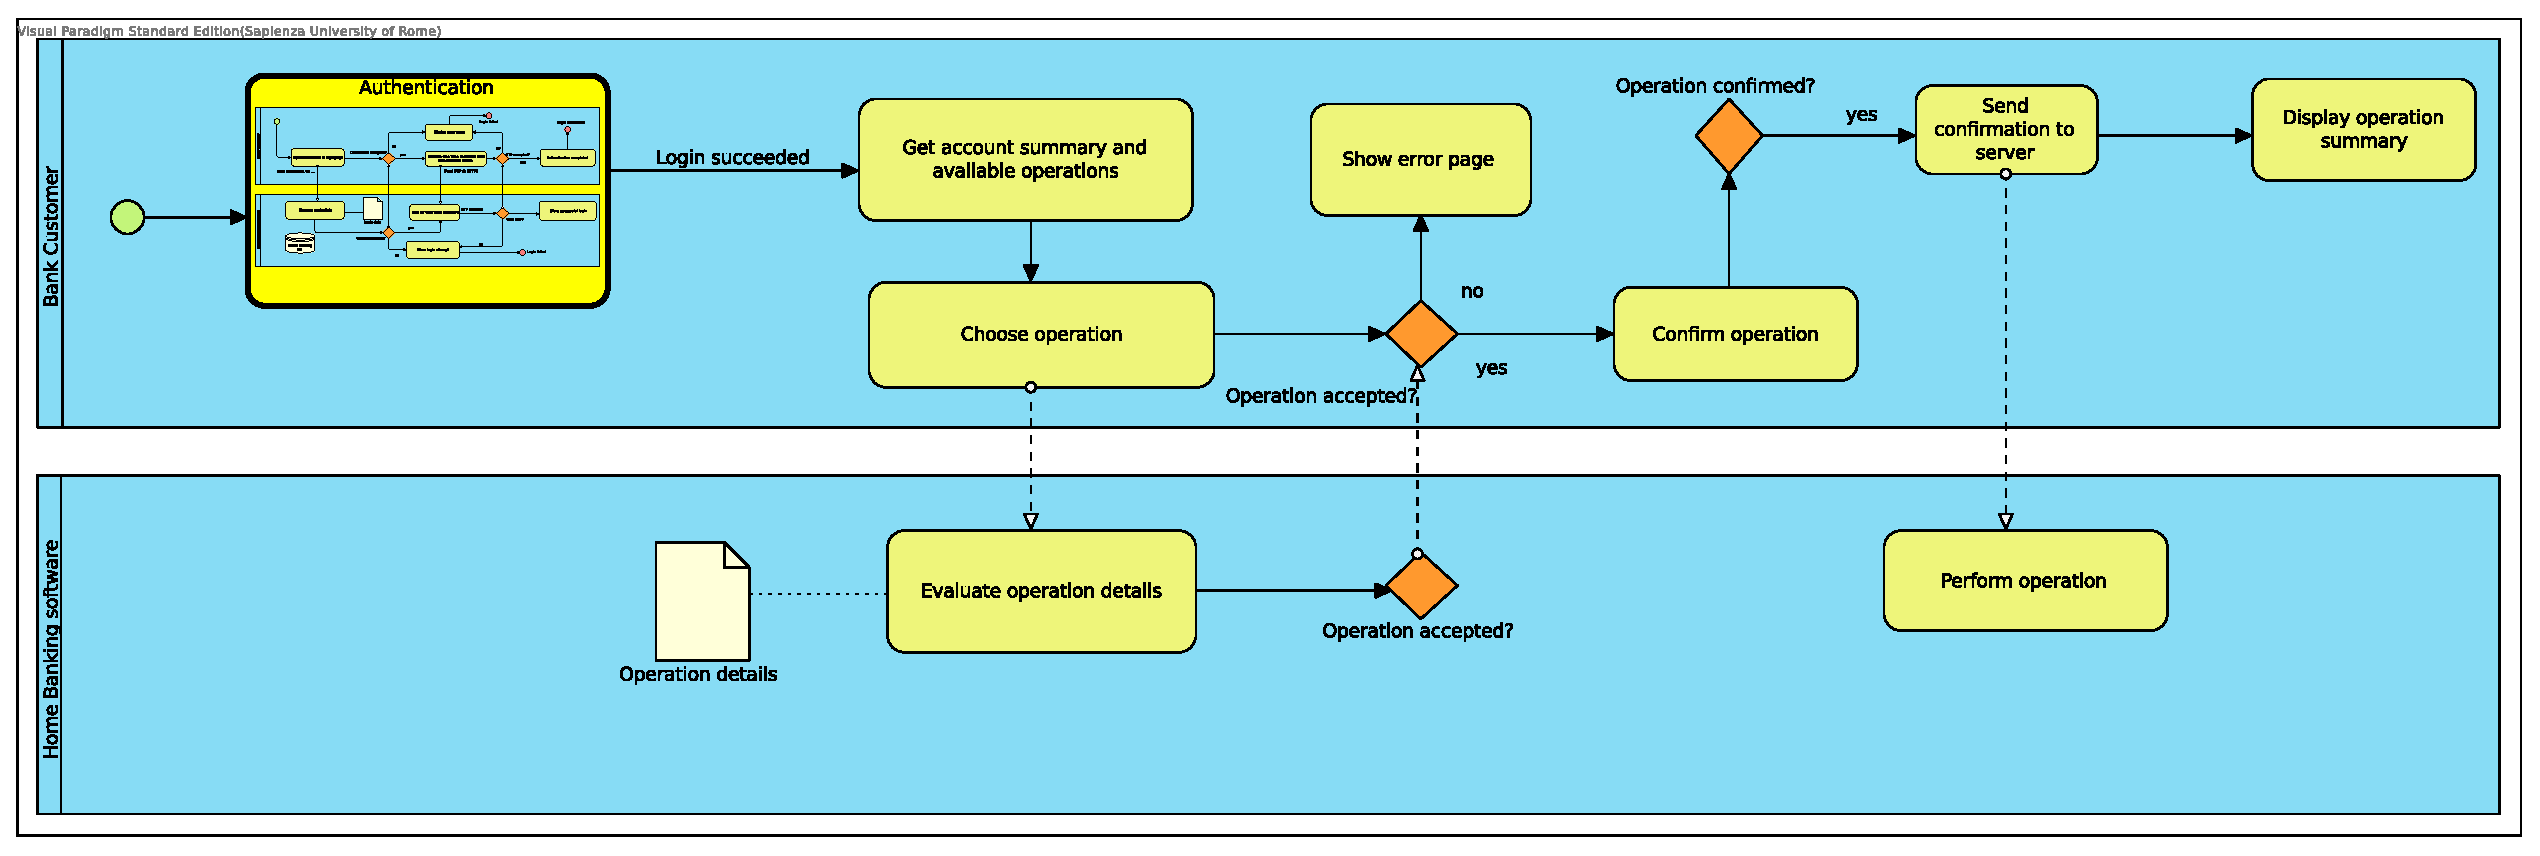
\includegraphics[width=\textheight, angle=90]{Images/Home_Banking_generic_action.eps}
	\caption{Business case: generica procedura di Home Banking effettuata da un utente del sistema.}
	\label{fig:business_case_generic_operation}
\end{figure*}

\end{document}
